\cvsection{Projects}

\begin{cventries}
  \cventry
    {} % Empty position
    {\,\faGithub\acvHeaderIconSep\href{https://github.com/BlackSamorez/ebanko}{NLP bot}} % Project
    {} % Empty location
    {} % Empty date
    {
      \begin{cvitems} % Description(s) bullet points
        \item {Telegram \textbf{bot} with \textbf{NLP} functionality}
        \item {Automatic \textbf{data collection} and preparation}
        \item {Easily deployed with \textbf{Docker compose}}
		\item {Full deployment with \textbf{Telegram API}, \textbf{backend} and \textbf{metrics}}
      \end{cvitems}
    }
    
  \cventry
    {} % Empty position
    {\,\faGithub\acvHeaderIconSep\href{https://github.com/BlackSamorez/raytracer21}{Raytracer}} % Project
    {} % Empty location
    {} % Empty date
    {
      \begin{cvitems} % Description(s) bullet points
        \item {An almost \textbf{pure C++ raytracing} program}
		\item {Features CATCH2 \textbf{unit tests} and \textbf{GitHub-CI}}
      \end{cvitems}
    }
    
  \cventry
    {ML design}
    {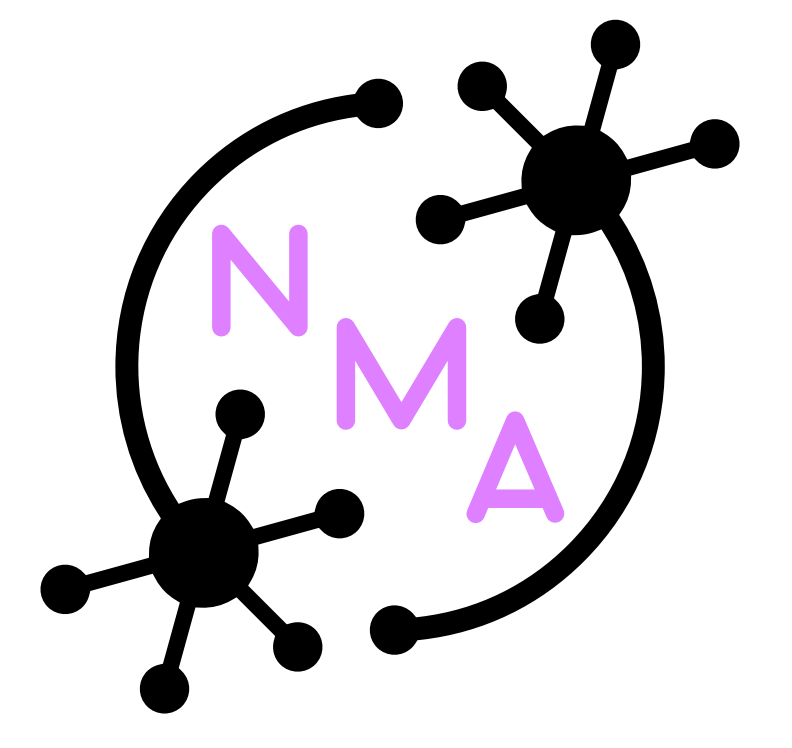
\includegraphics[width=3.5mm]{snippy-nma.png}\href{https://portal.neuromatchacademy.org/certificate/a6398835-adc9-4528-99d6-347675c05ffd}{Neuromatch Academy Final Project}}
    {}
    {Summer 2021}
    {
      \begin{cvitems}
        \item {Calcium imaging \textbf{neuron activity} analysis}
        \item {\textbf{Convolutional network} for \textbf{time series} analysis}
      \end{cvitems}
    }

\end{cventries}